\newif\ifvimbug
\vimbugfalse

\ifvimbug
\begin{document}
	\fi
\exercise{Pen \&  Paper Exercises: Learning Control Policies for Unknown Worlds}

\begin{questions}
	%----------------------------------------------
	
\begin{question}{The Bellman Equation for the State-Action Values}{2}

\begin{answer}
	
	The Bellman equation for the Q-function:
	$Q^\pi_{k+1} = R(s,a)+ \gamma\int P(s'|s,a) \int \pi(a',s') Q^\pi(s',a') da' ds'$
	% \sum_{s'}P(s'|s,a)V^\pi_k(s')$
	\\
	The equation is true for %todo[inline]{answer}
\end{answer}
\end{question}

\begin{question}{Vector-Matrix Notation of the Bellman Equation}{4}

\begin{answer}
	
	$q_{k+1}^\pi = r+ \gamma  P  (\Pi_\pi q_{k}^\pi)$
\end{answer}
\end{question}

\begin{question}{Towards a Continuous World}{1}
	
	\begin{answer}
		
		$Q^\pi(s,a) =\sum^{I}w_i  \Phi_i(s,a)$
	\end{answer}
\end{question}
	
\begin{question}{The Bellman Equation of the Approximate State-Action Value Function}{2}
	
	\begin{answer}
		
		$\Phi\omega = b + C\Phi\omega \Leftrightarrow \Phi\omega  = r(s,a) + \gamma P\Pi\Phi w$
	\end{answer}
\end{question}


\begin{question}{Derivation of the Parameters}{5}
	
	\begin{answer}
		\rotatebox{180}{
		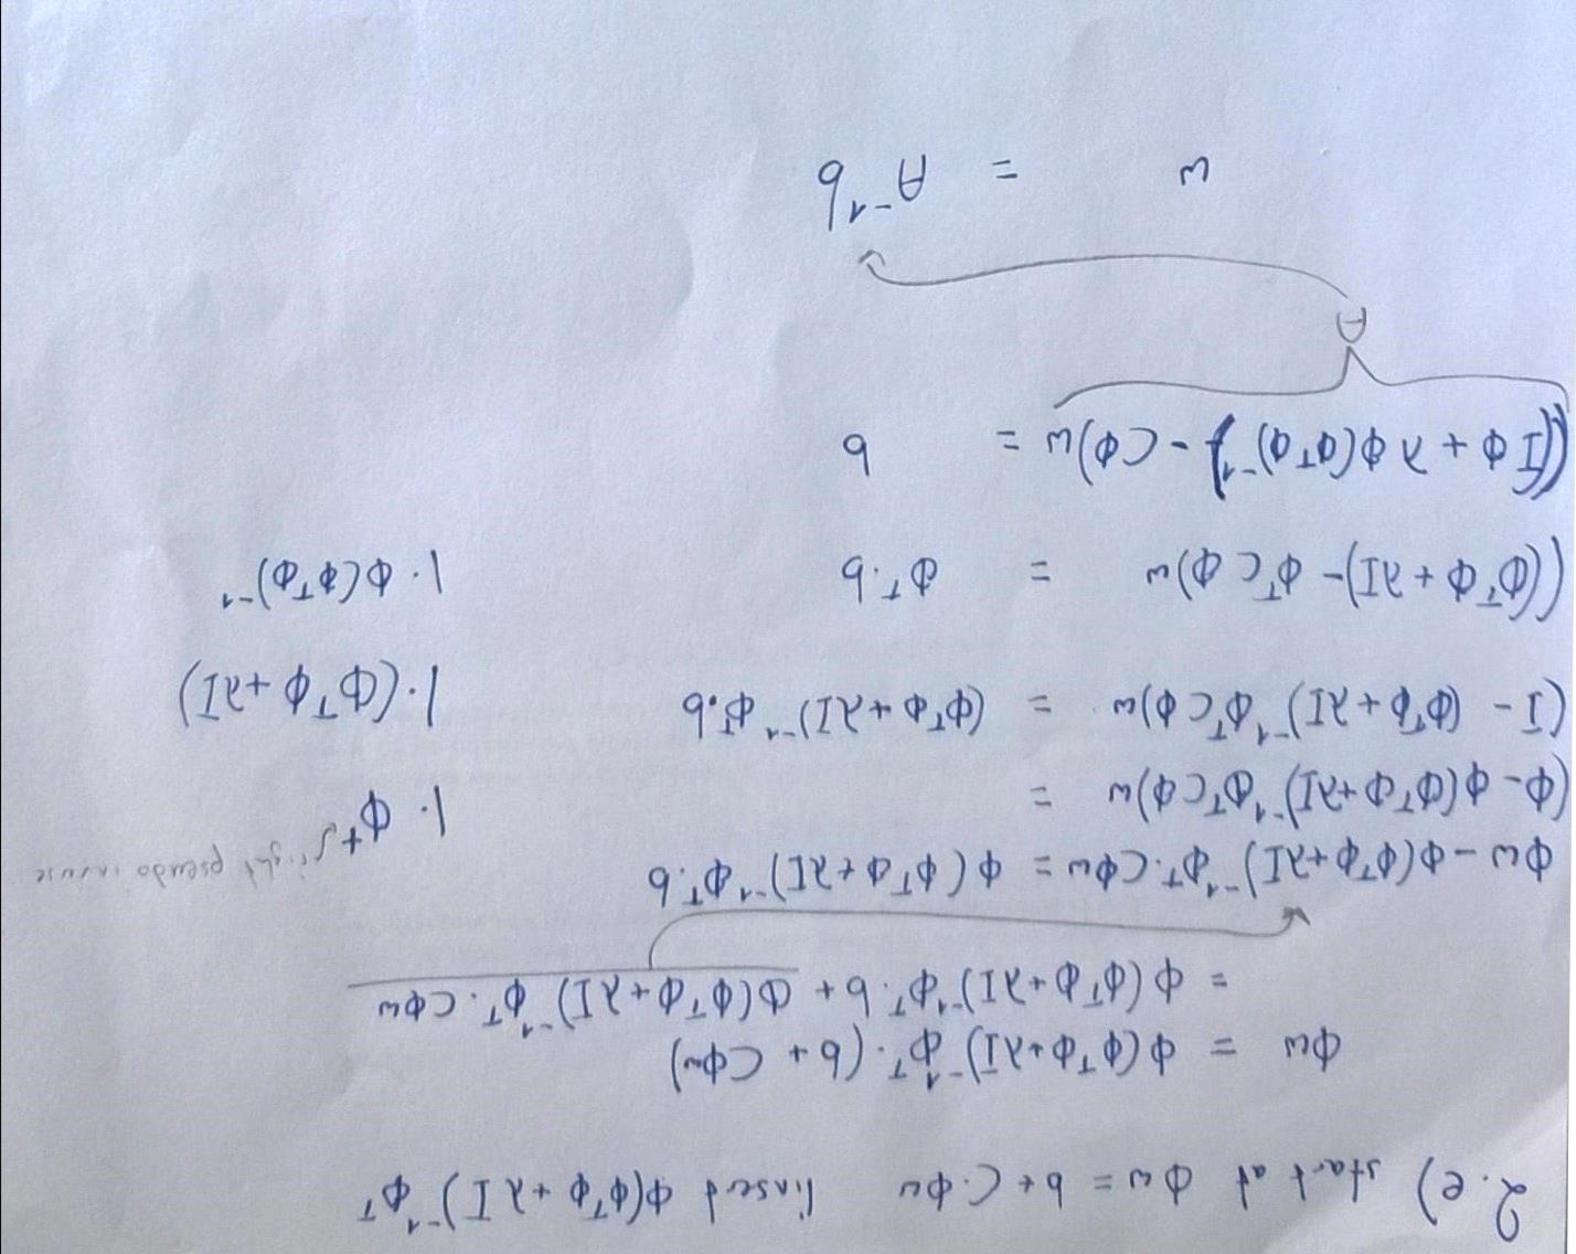
\includegraphics[width=\textwidth]{ImasHw32e.pdf}
	}
	\end{answer}
\end{question}

\begin{question}{Approaching the Algorithm}{5}
	
	Bonus Points question.
	\begin{answer}
		
		tbd
	\end{answer}
\end{question}


\begin{question}{Closing the Loop of the Algorithm}{5}
	
	\begin{answer}
		\begin{enumerate}
			\item	The analogue to computing the $\omega$ in the continuous case, is the policy evaluation (algorithm). [c.f. 05-Single Reinforcement Learning pp. 12-13]
			\item	We need to compute an update on $\omega$, an improvement.
			\item	Temporal differential update.
		\end{enumerate}

	\end{answer}
\end{question}

%----------------------------------------------
\end{questions}
